\section{USART}
All' interno del uC che stiamo vedendo ci sono 3 interfacce di comunicazione che riferiscono a 3 standard industriali differenti:
\begin{itemize}
    \item USART
    \item SPI
    \item I2C (anche conosciuta come TWI)
\end{itemize}

La USART è l' interfaccia di comunicazione più vecchia esistente, usa lo standard RS232.
E' molto utilizzato ancora oggi soprattutto per il debug: mentre il programma nel uC viene eseguito sulla linea seriale si stampano informazioni utili per monitorarne lo stato.

La velocità di comunicazione su questa linea si misura in baud dal nome dell' inventore di questo tipo di trasmissione.

La comunicazione binaria avviene per gruppetti di bit, di solito da 8 bit (1 byte).
Un singolo gruppetto viene anche chiamato \emph{frame}, il frame inoltre è composto, oltre che dal payload (cioè i dati che si vogliono comunicare) anche da alcuni bit ausiliari.

\subsection{Codifica}
Essendo un bit una entità astratta dobbiamo immaginare un modo di rappresentarlo fisicamente, possiamo pensare ad esempio a degli impulsi elettrici, questo processo è detto \emph{codifica}.
La codifica più elementare alla quale si può pensare è la seguente:
\begin{figure}[H]
    \centering
    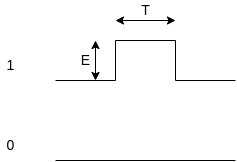
\includegraphics[width=150px]{images/22_USART/simple_bit_encoding.png}
\end{figure}
per comunicare quindi si pone E volt sulla linea per inviare 1 e si tiene la linea a 0V per inviare 0, T deve essere noto ad entrambi gli endpoint della comunicazione.
Questa codifica si chiama \emph{return to zero}.

\subsection{Inizio della comunicazione}
Il ricevitore in qualche modo dovrebbe riuscire a capire che si sta iniziando una nuova comunicazione, per fare ciò si può pensare di utilizzare un secondo collegamento ed usarlo come clock, tuttavia il clock va bene per comunicazioni a bassa distanza, quando le distanze diventano più grandi la sua efficacia cala drasticamente.
Vogliamo quindi una comunicazione senza clock, che ci permette anche di risparmiare questo collegamento.

\subsection{Potenza della trasmissione}
Il valore medio del segnale supponendo una comunicazione eterogenea di 0 al 50\% e di 1 al 50\% è $\frac{E}{2}$, trasmettendo segnali a media positiva ci sarà per forza una caduta di tensione che abbassa l' intensità del segnale e rende più complesso misurare correttamente.

\subsection{Codifica no return to zero}
\begin{figure}[H]
    \centering
    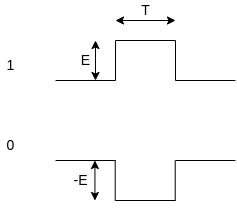
\includegraphics[width=150px]{images/22_USART/no_return_to_zero_encode.png}
\end{figure}
Questa codifica ci permette di risolvere il problema del valor medio, il problema dell' inizio della trasmissione ma non risolve il \emph{run-legth} cioè i bit tutti uguali che potrebbero far perdere la sincronizzazione tra trasmettitore e ricevitore.
Con questa codifica l' errore massimo ammesso in ricezione è il 6\%.

\subsection{Codifica Manchester}
\begin{figure}[H]
    \centering
    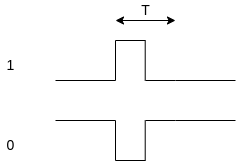
\includegraphics[width=150px]{images/22_USART/manchester_encoding.png}
\end{figure}
Questa codifica è immune agli errori di clock in quanto è autoclockante, in ogni periodo c'è una transizione che può essere utilizata per ri-sincronizzare trasmettitore e ricevitore.
E' anche detta \emph{modified frequency modulation}.
Un problema di questa codifica è che necessita di banda doppia per essere trasmessa.

\subsection{RS232}
Il protocollo RS232, sul quale si basa USART risolve i vari problemi incontrati in questa maniera:
\begin{itemize}
    \item in idle la linea è a 1
    \item quando si deve iniziare la comunicazione si porta giù la linea, questo è il bit di start e si usa per sincronizzare trasmettitore e ricevitore
    \item si inviano al massimo 9 bit di dato, in modo da non perdere la sincronizzazione
    \item alla fine si può inserire un bit di stop che è un bit ad 1
    \item prima di trasmettere altri dati bisogna aspettare del tempo
\end{itemize}
si cerca di campionare sempre a metà del picco quindi il primo campionamento è dopo $\frac{3T}{2}$ dalla ricezione dello start bit.

Le tensioni che si usano sono $\pm 7$V, la comunicazione è little endian quindi si trasmette dal bit meno significativo in poi.

Lo standard del protocollo non specifica quanto $T$ debba essere grande, però approva un largo insieme di valori $R = \frac{1}{T}$ detti \emph{baudrate}: 110, 300, 600, 1200, 2400, 4800, 9600, 19200, 38400, 57600, \_, 115200, ecc.
I più usati sono sicuramente 9600, 19200 e 115200.

La trasmissione è monodirezionale quindi per permettere a tutti e due gli endpoint di ricevere e trasmettere si usano due linee, alla fine i fili da collegare sono 3: TX, RX, GND.

\subsubsection{Implementazione in hardware}
In hardware possiamo implementare tutto con uno shift register a caricamento parallelo ed uscita seriale:
\begin{figure}[H]
    \centering
    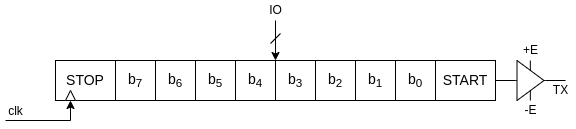
\includegraphics[width=300px]{images/22_USART/shift_register.png}
\end{figure}

Il ricevitore è implementato come un automa a stati finiti con velocità almeno di 16$R$ in modo da avere $\frac{T}{16}$ di periodo, con questa velocità posso permettermi di misurare il tempo necessario per campionare a metà del picco, inoltre posso eseguire 3 letture consecutive a ridosso del picco in modo da fare una media dei 3 valori per decidere quale valore si è letto.

Se nella triplice lettura dello stop bit ottengo di aver letto 0 invalido tutta la ricezione e segnalo un \emph{errore di trama}.

\subsection{USART nel uC}
Lo schema interno della periferica USART è:
\begin{figure}[H]
    \centering
    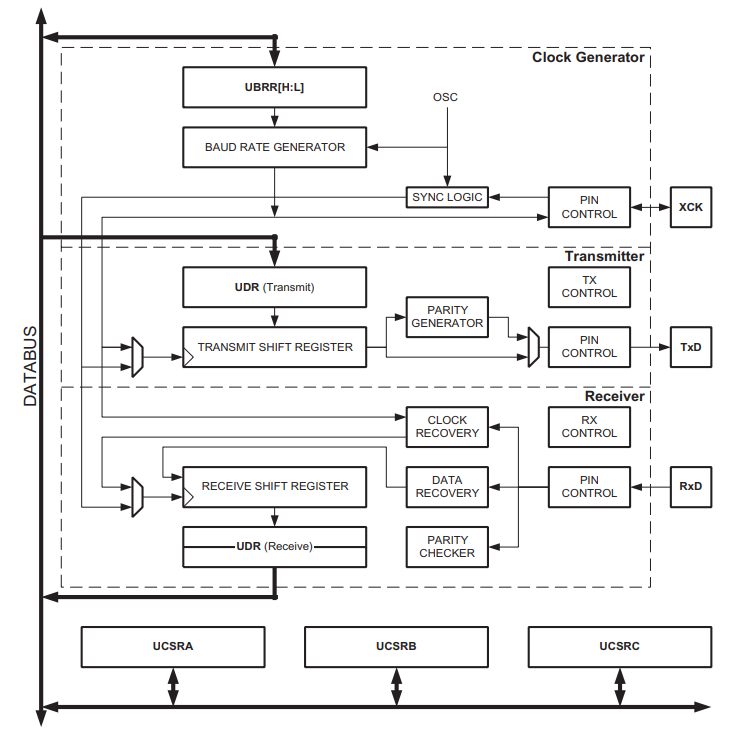
\includegraphics[width=300px]{images/22_USART/USART.png}
\end{figure}
Sia in ricezione che in trasmissione abbiamo 3 shift register che tengono in memoria fino a 3 byte con disciplina FIFO.

Abbiamo due principali modalità di funzionamento:
\begin{itemize}
    \item async: si trasmette un frame, si fa una pausa e ci si sincronizza ad ogni trama
    \item sync: è uno spreco di silicio
\end{itemize}

\subsubsection{UBRR}
Il registro UBRR è il prescaler del clock degli shift register, modificando il suo valore possiamo scegliere quale baudrate usare per le comunicazioni:
$$ UBRR = \frac{f_{OSC}}{16 \cdot BAUDRATE} -1 $$
$$ BAUDRATE = \frac{f_{OSC}}{16(UBRR + 1)} $$

\subsubsection{Formato del frame}
La periferica USART dell' ATMEGA32 ci permette di costruire una trama con:
\begin{itemize}
    \item start bit obbligatorio
    \item 5 bit di dati obbligatorio, ma possiamo inviarne fino a 9
    \item bit di parità pari opzionale
    \item bit di stop obbligatorio con un secondo bit di stop opzionale
\end{itemize}

\subsubsection{UDR - USART Data Register}
Questo singolo registro in realtà è mappato a due registri diversi in base al tipo di operazione.
Se stiamo leggendo leggiamo i dati ricevuti, se stiamo scrivendo invece scriviamo un dato da inviare.

\subsubsection{UCSRA}
\begin{figure}[H]
    \centering
    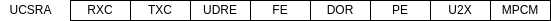
\includegraphics[width=320px]{images/22_USART/UCSRA.png}
\end{figure}
\begin{itemize}
    \item RXC: se c'è 1 è stata ricevuta una trama, all' accesso viene messo a 0 se ho svuotato la coda di ricezione
    \item TXC: se c'è 1 è stata trasmessa una trama, all' accesso viene messo a 0.
    In genere si guarda poco se non quando vogliamo spegnere la periferica USART e vogliamo accertarci di aver inviato tutti i dati
    \item UDRE: UDR empty, indica che c'è almeno un posto libero nella coda di trasmissione
    \item FE: frame error, indica che lo stop bit non tornava e quindi si deve ignorare il dato letto.
    In realtà sono due bit uno in coda all' altro in quanto ce n'è uno per ogni UDR
    \item DOR: data overrun, è ad 1 quando sono state ricevute più di 3 trame e quindi abbiamo perso qualcosa
    \item PE: parity error
    \item U2X: abilita la modalità fast
    \item MPCM: abilita la modalità di comunicazione multiprocessore
\end{itemize}

\subsubsection{UCSRB}
Contiene gli enabler delle varie interruzioni che riguardano la USART:
\begin{figure}[H]
    \centering
    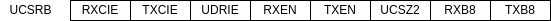
\includegraphics[width=320px]{images/22_USART/UCSRB.png}
\end{figure}
\begin{itemize}
    \item RXCIE: abilita l' interrupt sulla ricezione
    \item TXCIE: abilità l' interrupt sulla trasmissione
    \item UDRIE: abilita l' interrupt sulla coda vuota
    \item RXEN: abilita il ricevitore
    \item TXEN: abilita il trasmettitore
    \item UCSZ0/1/2: si usa per indicare la lunghezza del frame
    \item RXB8: contiene il 9 bit ricevuto se si usa una trama a 9 bit
    \item TXB8: ci si inserisce il 9 bit da trasmettere se si usa una trama a 9 bit
\end{itemize}

\subsubsection{UCSRC}
\begin{figure}[H]
    \centering
    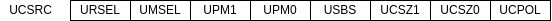
\includegraphics[width=320px]{images/22_USART/UCSRC.png}
\end{figure}
\begin{itemize}
    \item URSEL: se alla scrittura il suo valore è 1 allora la scrittura avverrà in UCSRC, se alla scrittura il valore è 0 allora stiamo scrivendo in UBRRH
    \item UPM0/1: si usano per impostare il tipo di parità da usare
    \item USBS: si usa per indicare quanti bit di stop si devono usare
\end{itemize}

\subsubsection{UBRRL/UBRRH}
E' il prescaler del clock degli shift register.


